% Provenance (never printed): see sources/outline_sources.md (Year 3:
% moments of inertia and gravity fields; impact cratering and crater dating;
% volcanism and tectonics on Mars, Venus, Io and the icy moons).
% Brief: sources/book5/BRIEFS.md, ch. 26. Curves from figdata/bachelor-3/
% two_layer_planet.py (two-layer interiors of the Earth, Mars, the Moon and
% Mercury from mean density and moment of inertia) and crater_sfd.py
% (the Ivanov production function and the Hartmann-Neukum chronology of
% Mars from the Craterstats configuration, the lunar chronology of Neukum,
% Hartmann's equilibrium density, and two invented Martian plains whose
% counts are drawn once from a Poisson law). Exercise and problem values in
% the Book 5 scratch calculator calc/ch26.py. Plains A and B are invented.
\chapter{Interiores e superfícies planetárias}\label{ch:b3:planetary-interiors-surfaces}

Observada com binóculos, a Lua tem dois tipos de terreno. As terras altas
claras estão cobertas de crateras, uma sobre a outra: foram saturadas
com crateras grandes por um intenso bombardeio que terminou há cerca de 3.8 bilhões
de anos atrás. Os mares escuros, planícies preenchidas por lava entre 4.2 e 1.2
bilhão de anos atrás, têm muito menos crateras. As missões Apollo e Luna
trouxeram rochas de ambos, e suas idades radiométricas transformaram a
densidade de crateras sobre uma superfície em um relógio. Hoje o relógio data
planícies em Marte, Mercúrio e nas luas geladas, das quais nenhuma rocha foi
trazida até agora. Este capítulo lê os interiores dos planetas em sua
gravidade, rotação e marés, e depois suas superfícies em suas crateras,
vulcões e falhas.
% ledger: french:highlands, nasa:moon-core, marchi:neukum

\begin{recall}
O fator de momento de inércia $C = I/MR^2$, o modelo de duas camadas de um planeta
construído a partir dele e da densidade média, os planetas terrestres e os
gigantes estão no volume do primeiro ano, em seu capítulo sobre
planetologia comparada; as plumas do manto e as grandes províncias ígneas, em seu capítulo sobre
pontos quentes. A diferenciação planetária e os meteoritos estão no volume do segundo
ano, em seu capítulo sobre formação planetária. O \omterm{def:b3:gravity-geodesy:j2}{fator de forma dinâmico}
$J_2$, a \omterm{thm:b3:gravity-geodesy:maccullagh}{fórmula de MacCullagh} e a flexura da litosfera estão neste
volume, em seu capítulo sobre gravidade e geodésia; o \omterm{def:b3:mantle-convection:rayleigh}{número de Rayleigh}, em seu
capítulo sobre convecção do manto. Marés, leis de Kepler e módulos elásticos
estão nos livros de física; a distribuição de Poisson, nos livros de
matemática.
\end{recall}

\section{Interiores a partir da gravidade, rotação e marés}\label{sec:b3:planetary-interiors-surfaces:interiors}

A massa de um planeta, obtida a partir da órbita de uma lua ou de uma sonda, fornece sua
densidade média; a precessão de seu eixo e seu $J_2$ fornecem seu momento de
inércia. O modelo de duas camadas do volume do primeiro ano transforma os dois
números em um núcleo, mas somente depois de escolhida uma densidade do manto: duas
medidas não podem determinar três incógnitas.

\begin{omfigure}
\centering
\begin{tikzpicture}
\begin{axis}[width=0.78\linewidth, height=0.46\linewidth,
  xmin=3000, xmax=16000, ymin=0, ymax=1,
  xlabel={densidade do núcleo $\rho_c$ (\unit{kg.m^{-3}})},
  ylabel={raio do núcleo / raio do planeta $x$},
  tick label style={font=\scriptsize}, label style={font=\small},
  scaled x ticks=false, xtick={4000,6000,8000,10000,12000,14000,16000},
  xticklabels={4000,6000,8000,10\,000,12\,000,14\,000,16\,000}]
\addplot[thick, omDef] table[x=rho_c, y=x] {figdata/out/bachelor-3-two_layer_planet-curve-Earth.dat};
\addplot[thick, red!70!black] table[x=rho_c, y=x] {figdata/out/bachelor-3-two_layer_planet-curve-Mars.dat};
\addplot[thick, black!60, dashed] table[x=rho_c, y=x] {figdata/out/bachelor-3-two_layer_planet-curve-Moon.dat};
\addplot[thick, orange!80!black] table[x=rho_c, y=x] {figdata/out/bachelor-3-two_layer_planet-curve-Mercury.dat};
\addplot[only marks, mark=*, mark size=2pt, black] table[x=rho_c, y=x] {figdata/out/bachelor-3-two_layer_planet-points.dat};
\node[font=\scriptsize, omDef, anchor=south west] at (axis cs:12600,0.55) {Terra};
\node[font=\scriptsize, red!70!black, anchor=south west] at (axis cs:6600,0.55) {Marte};
\node[font=\scriptsize, black!70, anchor=south west] at (axis cs:11000,0.2) {Lua};
\node[font=\scriptsize, orange!80!black, anchor=south west] at (axis cs:7300,0.83) {Mercúrio};
\end{axis}
\end{tikzpicture}
\par\smallskip{\small Os modelos de duas camadas permitidos pela densidade média e
o fator de momento de inércia de quatro corpos: cada curva percorre as
possíveis densidades do manto, um manto mais denso deixando um núcleo menor e mais
denso. Os pontos marcam os raios medidos do núcleo: o da Terra, a partir da sismologia;
o de Marte, a partir do sismômetro da InSight; o núcleo interno e a
camada líquida da Lua; o de Mercúrio, a partir do campo gravitacional da
sonda MESSENGER.}\label{fig:b3:planetary-interiors-surfaces:two-layer}
\end{omfigure}
% ledger: planet:Earth.density, planet:Mars.density, planet:Moon.density, planet:Mercury.density, earth:MoI, nasa:mars, nasa:moon, nasa:mercury, data:prem, jpl:insight-interior, nasa:moon-core, agu:mercury-core

Cada planeta fornece uma curva, não um ponto. Para Marte, o raio do núcleo de
\qty{1830}{km} medido pela InSight escolhe um manto de \qty{3460}{kg.m^{-3}}
e um núcleo de \qty{6460}{kg.m^{-3}}. Para Mercúrio, o núcleo de cerca de
\qty{2000}{km} de raio ocupa 82 por cento do raio. A curva da Lua é
quase plana: seu $C = 0.394$ está tão próximo de $\tfrac25$ que um núcleo pequeno
de qualquer densidade se ajusta, e uma variação de $0.001$ em $C$ desloca o raio
do núcleo por mais de um fator de dois (\cref{exo:b3:planetary-interiors-surfaces:10}).
A gravidade, sozinha, não enxerga um núcleo pequeno; as marés e as ondas sísmicas, sim.
% ledger: jpl:insight-interior, agu:mercury-core, nasa:moon

\begin{definition}[Número de Love]\label{def:b3:planetary-interiors-surfaces:love-number}
Quando um potencial de maré de grau~2 atua sobre um planeta, o planeta se deforma e
sua massa redistribuída acrescenta um potencial próprio. O \emph{número
de Love}\index{número de Love} $k_2$ é a razão entre esse potencial acrescentado e o
potencial de maré, ambos tomados na superfície do planeta.
\end{definition}

Um planeta rígido tem $k_2 = 0$; um planeta fluido de densidade uniforme cede
totalmente, com $k_2 = \tfrac32$. Entre os dois extremos, o número mede
quanto do planeta cede.

\begin{proposition}[Número de Love de uma esfera elástica uniforme]\label{prop:b3:planetary-interiors-surfaces:kelvin}
Uma esfera incompressível de densidade uniforme $\rho$, raio $R$, gravidade
superficial $g$ e rigidez $\mu$ tem
\[
  k_2 = \frac{3/2}{1 + \dfrac{19\mu}{2\rho g R}} .
\]
\end{proposition}

O resultado, devido a Kelvin, é admitido. A razão $\mu/\rho gR$ compara
a rigidez elástica com a autogravidade que puxa a protuberância de maré
de volta: planetas pequenos são rígidos, os grandes cedem. Para Marte, $\rho gR =
\qty{4.97e10}{Pa}$; com a rigidez do manto superior da Terra,
\qty{67}{GPa} a \qty{80}{km} de profundidade no modelo de referência da Terra, a
fórmula dá $k_2 = 0.109$. O rastreamento da sonda Mars Global Surveyor
em órbita mediu a maré solar de Marte: $k_2 = 0.153 \pm 0.017$, grande demais
para um núcleo sólido de ferro. Pelo menos a parte externa do núcleo é
líquida, e seu raio foi situado entre 1520 e \qty{1840}{km} em 2003.
% ledger: nasa:mars, const:G, data:prem, yoder:mars-k2

Sismômetros resolveram a questão. A sonda InSight registrou
marsismos e detectou ondas refletidas do topo do núcleo: raio
\qty{1830}{km}, sob um manto com \qty{1560}{km} de profundidade e uma crosta de 20 a
\qty{37}{km} de espessura. Na Lua, os sismômetros instalados pelos astronautas da Apollo
registraram luassismos, os mais profundos deles, a centenas de
quilômetros de profundidade, desencadeados pelas marés terrestres. O núcleo da Lua é agora
descrito como um núcleo interno sólido, rico em ferro, com \qty{240}{km} de raio, uma
camada líquida de ferro com \qty{90}{km} de espessura ao seu redor, e uma
camada parcialmente fundida acima.
% ledger: jpl:insight-interior, nasa:moonquakes, nasa:moon-core

\section{Crateras de impacto}\label{sec:b3:planetary-interiors-surfaces:impacts}

Um corpo vindo do espaço atinge um planeta com velocidade não inferior à de escape do planeta
de escape, \qty{11.2}{km.s^{-1}} no caso da Terra; asteroides costumam atingir a Terra
a 15 a \qty{25}{km.s^{-1}}, e cometas, a até
\qty{60}{km.s^{-1}}. A \qty{20}{km.s^{-1}}, cada quilograma carrega
\qty{2e8}{J}, cerca de cinquenta vezes a energia de um quilograma de explosivo. O
impacto envia uma onda de choque para o solo e para o projétil, que
se funde e vaporiza; atrás do choque, a rocha é posta em movimento para fora e
uma cratera se abre em segundos.
% ledger: french:velocities, french:table21

\begin{definition}[Cratera transitória, cratera simples, cratera complexa, manto de ejetos]\label{def:b3:planetary-interiors-surfaces:crater-morphology}
A \emph{cratera transitória}\index{cratera transitória} é a cavidade em forma de tigela
aberta pelo fluxo de escavação no instante em que deixa de crescer; sua
profundidade é cerca de um terço do diâmetro. Uma \emph{cratera
simples}\index{cratera simples} é uma tigela com borda elevada, a cratera transitória
praticamente sem alteração: suas paredes íngremes desabam para dentro, formando uma lente de
brecha. Uma \emph{cratera complexa}\index{cratera complexa} é uma cratera maior
cuja tigela transitória colapsou: o piso se elevou formando um soerguimento central, a
borda deslizou para dentro ao longo de terraços, e o piso é plano. O \emph{manto de
ejetos}\index{manto de ejetos} é a camada de rocha escavada lançada para fora
além da borda e depositada ao redor da cratera.
\end{definition}
% ledger: french:transient, french:transition

\begin{omfigure}
\centering
\begin{tikzpicture}[x=0.55cm, y=0.55cm, font=\scriptsize, >=stealth]
\def\simpleprofile{(-6,0) -- (-3.6,0) .. controls (-3.0,0.45) .. (-2.6,0.55) .. controls (-1.8,-2.6) and (1.8,-2.6) .. (2.6,0.55) .. controls (3.0,0.45) .. (3.6,0) -- (6,0)}
\def\complexprofile{(-7,0) -- (-5.4,0) -- (-4.6,0.5) -- (-4.0,-0.3) -- (-3.6,-0.25) -- (-3.1,-1.0) -- (-2.7,-0.95) -- (-2.3,-1.5) -- (-0.8,-1.5) -- (-0.5,-0.6) -- (0,-0.3) -- (0.5,-0.6) -- (0.8,-1.5) -- (2.3,-1.5) -- (2.7,-0.95) -- (3.1,-1.0) -- (3.6,-0.25) -- (4.0,-0.3) -- (4.6,0.5) -- (5.4,0) -- (7,0)}
\begin{scope}
\fill[black!8] \simpleprofile -- (6,-4) -- (-6,-4) -- cycle;
\begin{scope}
\clip \simpleprofile -- (6,-4) -- (-6,-4) -- cycle;
\draw[black!45] (-6,-1.2) -- (6,-1.2) (-6,-2.4) -- (6,-2.4);
\fill[black!28] (-2.25,-0.5) .. controls (-1.2,-2.05) and (1.2,-2.05) .. (2.25,-0.5) .. controls (1.0,-0.8) and (-1.0,-0.8) .. (-2.25,-0.5);
\end{scope}
\fill[black!40] (-5.2,0) -- (-2.6,0.55) -- (-3.6,0.12) -- cycle;
\fill[black!40] (5.2,0) -- (2.6,0.55) -- (3.6,0.12) -- cycle;
\draw[thick] \simpleprofile;
\draw[omDef, dashed, thick] (-2.4,0.35) .. controls (-1.6,-3.1) and (1.6,-3.1) .. (2.4,0.35);
\node[anchor=south] at (0,1.2) {cratera simples};
\node[fill=black!28, inner sep=1pt] at (0,-1.45) {lente de brecha};
\node[omDef, anchor=north, fill=black!8, inner sep=1pt] at (0,-2.65) {cratera transitória};
\draw[->] (-4.9,1.2) node[anchor=south] {ejetos} -- (-4.3,0.2);
\draw[->] (3.6,1.4) node[anchor=south] {borda elevada} -- (2.8,0.62);
\end{scope}
\begin{scope}[xshift=7.6cm]
\fill[black!8] \complexprofile -- (7,-4) -- (-7,-4) -- cycle;
\begin{scope}
\clip \complexprofile -- (7,-4) -- (-7,-4) -- cycle;
\draw[black!45] (-7,-1.2) -- (7,-1.2);
\draw[black!45] (-7,-2.4) -- (-1.3,-2.4) .. controls (-0.6,-2.4) and (-0.5,-1.75) .. (0,-1.75) .. controls (0.5,-1.75) and (0.6,-2.4) .. (1.3,-2.4) -- (7,-2.4);
\draw[black!45] (-7,-3.4) -- (-1.6,-3.4) .. controls (-0.7,-3.4) and (-0.6,-2.7) .. (0,-2.7) .. controls (0.6,-2.7) and (0.7,-3.4) .. (1.6,-3.4) -- (7,-3.4);
\draw[black!70] (-4.0,-0.3) -- (-3.2,-2.0) (4.0,-0.3) -- (3.2,-2.0) (-3.1,-1.0) -- (-2.5,-2.2) (3.1,-1.0) -- (2.5,-2.2);
\end{scope}
\draw[thick] \complexprofile;
\node[anchor=south] at (0,1.5) {cratera complexa};
\draw[->] (1.4,0.75) node[anchor=south west, inner sep=1pt] {soerguimento central} -- (0.25,-0.2);
\node[anchor=north, fill=black!8, inner sep=0.5pt] at (-1.3,-1.6) {piso plano};
\draw[->] (-3.2,1.4) node[anchor=south] {terraços} -- (-3.8,-0.12);
\draw[->] (-5.6,-0.6) node[anchor=east, fill=black!8, inner sep=1pt, xshift=4pt] {falhas} -- (-3.65,-1.35);
\node[anchor=north, fill=black!8, inner sep=1pt] at (0,-3.55) {camadas soerguidas};
\end{scope}
\end{tikzpicture}
\par\smallskip{\small Seções transversais de uma \omterm{def:b3:planetary-interiors-surfaces:crater-morphology}{cratera simples} e de uma \omterm{def:b3:planetary-interiors-surfaces:crater-morphology}{cratera complexa} em
rocha estratificada (sem escala). À esquerda: a tigela de uma \omterm{def:b3:planetary-interiors-surfaces:crater-morphology}{cratera simples} mantém a
forma da \omterm{def:b3:planetary-interiors-surfaces:crater-morphology}{cratera transitória} (tracejada), parcialmente preenchida por uma lente de brecha,
sob uma borda elevada e um \omterm{def:b3:planetary-interiors-surfaces:crater-morphology}{manto de ejetos}. À direita: numa \omterm{def:b3:planetary-interiors-surfaces:crater-morphology}{cratera complexa}, a
tigela transitória colapsou; as camadas profundas subiram sob um
soerguimento central, e a borda deslizou para dentro ao longo de falhas, formando
terraços.}\label{fig:b3:planetary-interiors-surfaces:craters}
\end{omfigure}
% ledger: french:transient, french:transition

\begin{omfigure}
\centering
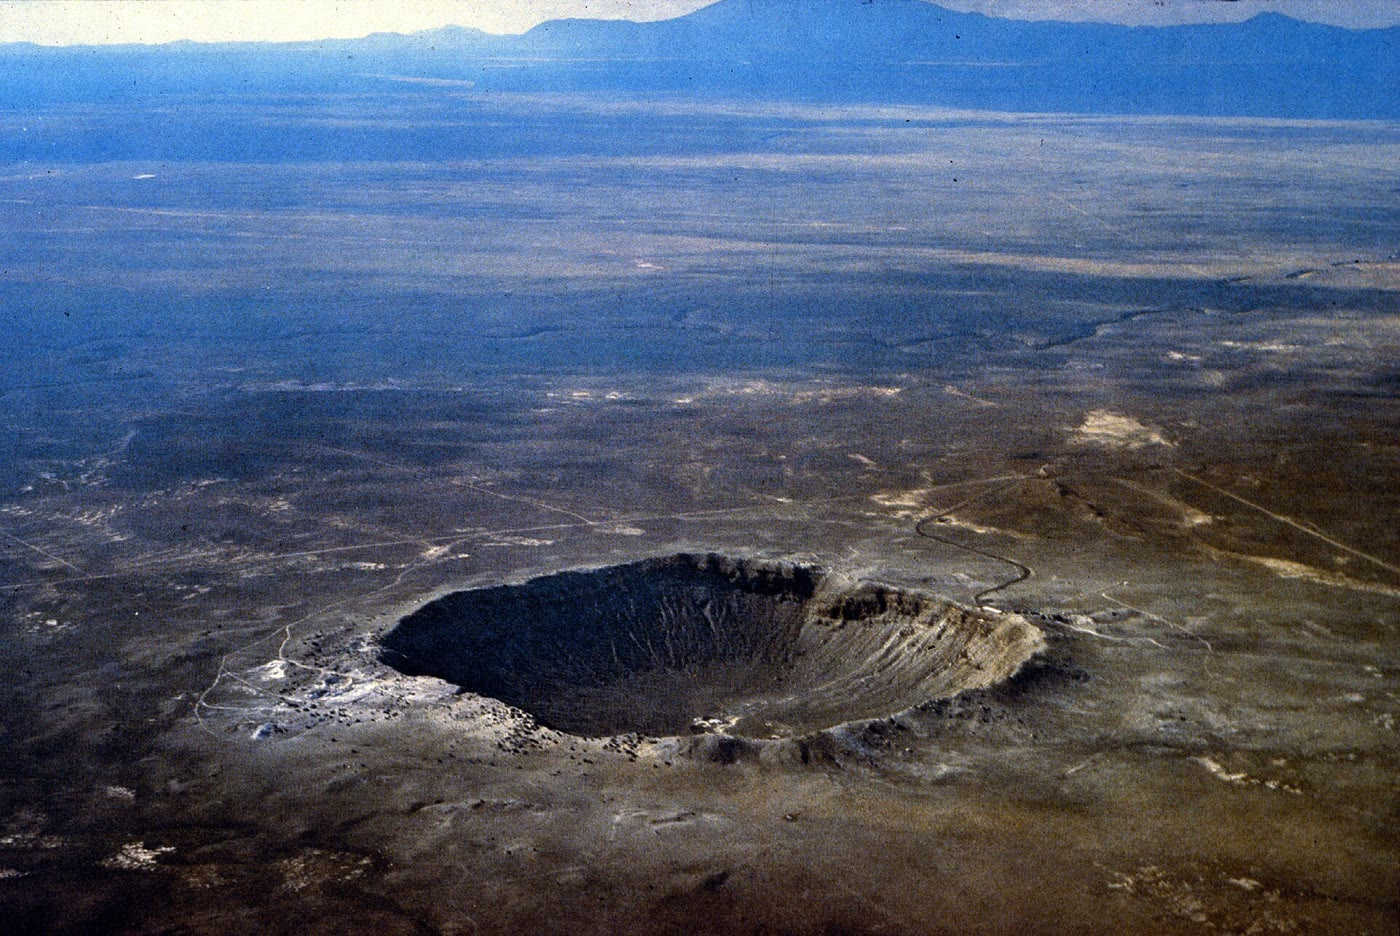
\includegraphics[width=0.66\linewidth]{images/book5/b3-barringer-crater.jpg}
\par\smallskip{\small Barringer Meteor Crater, Arizona, uma \omterm{def:b3:planetary-interiors-surfaces:crater-morphology}{cratera simples}
com \qty{1.2}{km} de diâmetro, formada há cerca de 50,000 anos por um meteorito de ferro
com cerca de \qty{30}{m} de diâmetro; a borda se ergue acima do planalto, e o \omterm{def:b3:planetary-interiors-surfaces:crater-morphology}{manto de ejetos}
se espalha ao seu redor. Fotografia aérea, USGS/D.~Roddy, domínio
público.}\label{fig:b3:planetary-interiors-surfaces:barringer}
\end{omfigure}
% ledger: photo:b3-barringer, french:barringer

A escavação de uma cratera de \qty{1}{km} de diâmetro leva cerca de seis segundos; a de uma cratera de
\qty{200}{km} de diâmetro, cerca de um minuto e meio. O tamanho da
cratera que um impacto produz depende da energia do projétil, da gravidade e
da resistência da rocha; as leis que os relacionam são ajustadas a
experimentos e explosões, na forma de produtos de grupos adimensionais,
e são admitidas aqui. Seu espírito está num balanço de energias.
% ledger: french:transient

\begin{proposition}[Escalonamento no regime gravitacional]\label{prop:b3:planetary-interiors-surfaces:scaling}
Se uma fração fixa da energia do impacto $E$ eleva a rocha escavada, de
densidade $\rho$, contra a gravidade $g$, o diâmetro da cratera cresce como
\[
  D \propto \left(\frac{E}{\rho g}\right)^{1/4} .
\]
\end{proposition}

\begin{proof}
O volume escavado escala como $D^3$, sua massa como $\rho D^3$, e ele é
elevado a uma altura da ordem de $D$: o trabalho é da ordem de $\rho g D^4$, que
é proporcional a $E$.
\end{proof}

Parte da energia vai para calor, fusão e ruptura da rocha, de modo que as
leis reais ficam entre esta e regras mais simples: uma tabela frequentemente
citada para a Terra fornece uma cratera vinte vezes mais larga que o seu
projétil rochoso. A gravidade também define onde uma cratera deixa de ser simples. As
paredes da cavidade transitória desabam quando o peso da rocha que elas sustentam,
da ordem de $\rho g D/3$, supera a resistência da rocha, de modo que o
diâmetro de transição varia como $1/g$: cerca de \qty{4}{km} em rocha cristalina
e \qty{2}{km} em sedimentos na Terra, cerca de \qty{20}{km} na
Lua, onde a gravidade é seis vezes mais fraca.
% ledger: french:table21, french:transition, planet:Earth.gravity, planet:Moon.gravity

\section{Datação por crateras}\label{sec:b3:planetary-interiors-surfaces:dating}

Uma superfície deixada em repouso acumula crateras na taxa em que corpos a
atingem. Contá-las data a superfície, desde que a taxa seja conhecida e que as
crateras sejam da própria superfície, e não do que jaz abaixo ou dos
detritos lançados por um vizinho.

\begin{definition}[Distribuição tamanho--frequência das crateras]\label{def:b3:planetary-interiors-surfaces:sfd}
A \emph{distribuição tamanho--frequência das crateras}\index{distribuição tamanho--frequência das crateras}
de uma superfície é o número $N(D)$ de crateras de diâmetro de pelo menos $D$ por
unidade de área, em função de $D$ (a distribuição cumulativa), ou os
números contados em intervalos de diâmetro, geralmente cada um $\sqrt2$ vezes mais largo
que o anterior (a distribuição incremental).
\end{definition}

\begin{definition}[Datação por crateras; funções de produção e de cronologia; densidade de equilíbrio]\label{def:b3:planetary-interiors-surfaces:crater-dating}
A \emph{datação por crateras}\index{datação por crateras} é a determinação da idade
de uma superfície a partir da densidade de suas crateras. A \emph{função de produção
de crateras}\index{função de produção de crateras} é a forma da
\omterm{def:b3:planetary-interiors-surfaces:sfd}{distribuição tamanho--frequência das crateras} que uma superfície adquire, $F(D) =
N(D)/N(\qty{1}{km})$, supondo-se a mesma em todas as idades. A \emph{função de cronologia
de crateras}\index{função de cronologia de crateras} $N_1(T)$ é o
número de crateras de \qty{1}{km} ou mais por unidade de área acumuladas em um
tempo $T$. Uma superfície está na \emph{densidade de equilíbrio de
crateras}\index{densidade de equilíbrio de crateras} para crateras de um dado
tamanho quando cada nova cratera apaga, em média, tantas antigas quanto acrescenta:
seu número deixa de crescer.
\end{definition}

A idade-modelo de uma superfície decorre de uma única contagem: $N(D)$ medido em qualquer
$D$ fornece $N_1 = N(D)/F(D)$, e $T$ resolve $N_1(T) = N_1$. As retas
$N(D) = N_1(T)F(D)$ para $T$ fixo são chamadas isócronas. Para Marte, uma
função de produção muito usada é um polinômio de grau~11 em $\log_{10}D$, e a
função de cronologia tem a forma
\[
  N_1(T) = a\left(e^{bT} - 1\right) + cT , \qquad
  a = \qty{3.22e-14}{km^{-2}}, \ b = \qty{6.93}{Ga^{-1}}, \
  c = \qty{4.875e-4}{km^{-2}.Ga^{-1}} ,
\]
linear nos últimos três bilhões de anos, e fortemente exponencial antes. A
função da Lua tem a mesma forma, com $a = \num{5.44e-14}$ e $c =
\num{8.38e-4}$. Ela foi ajustada às idades dos sítios de pouso das missões Apollo e Luna;
a de Marte é a da Lua, reescalonada por uma estimativa da razão entre as taxas de
formação de crateras em Marte e na Lua.
% ledger: craterstats:mars-pf, craterstats:mars-cf, craterstats:moon-cf, marchi:neukum

\begin{omfigure}
\centering
\begin{tikzpicture}
\begin{groupplot}[group style={group size=2 by 1, horizontal sep=1.6cm},
  width=0.48\linewidth, height=0.46\linewidth,
  tick label style={font=\scriptsize}, label style={font=\small}, title style={font=\small}]
\nextgroupplot[title={isócronas em Marte}, xmode=log, ymode=log, xmin=0.1, xmax=100,
  ymin=1e-8, ymax=100, xlabel={diâmetro da cratera $D$ (\unit{km})},
  ylabel={$N(D)$, crateras $\geq D$ por \unit{km^2}},
  xtick={0.1,1,10,100}, xticklabels={0.1,1,10,100},
  ytick={1e-8,1e-6,1e-4,1e-2,1}]
\addplot[thick, black!50, dashed] table[x=D, y=eq] {figdata/out/bachelor-3-crater_sfd-iso.dat};
\addplot[omDef] table[x=D, y=N_0.1] {figdata/out/bachelor-3-crater_sfd-iso.dat};
\addplot[omDef] table[x=D, y=N_1] {figdata/out/bachelor-3-crater_sfd-iso.dat};
\addplot[omDef] table[x=D, y=N_3.5] {figdata/out/bachelor-3-crater_sfd-iso.dat};
\addplot[red!70!black, thick] table[x=D, y=N_4] {figdata/out/bachelor-3-crater_sfd-iso.dat};
\node[font=\tiny, omDef, anchor=north east] at (axis cs:0.75,8e-6) {0.1~Ga};
\node[font=\tiny, omDef, anchor=north east] at (axis cs:2.6,1e-5) {1~Ga};
\node[font=\tiny, omDef, anchor=north east] at (axis cs:9,3.5e-5) {3.5~Ga};
\node[font=\tiny, red!70!black, anchor=north east] at (axis cs:45,2.5e-5) {4~Ga};
\node[font=\tiny, black!60, anchor=south, rotate=-30] at (axis cs:25,3.5e-4) {equilíbrio};
\nextgroupplot[title={funções de cronologia}, ymode=log, xmin=0, xmax=4.5,
  ymin=1e-5, ymax=0.3, xlabel={idade $T$ (\unit{Ga})}, ylabel={$N_1$ por \unit{km^2}},
  legend style={font=\scriptsize, at={(0.03,0.97)}, anchor=north west}]
\addplot[thick, red!70!black] table[x=T, y=mars] {figdata/out/bachelor-3-crater_sfd-chron.dat};
\addlegendentry{Marte}
\addplot[thick, black!60, dashed] table[x=T, y=moon] {figdata/out/bachelor-3-crater_sfd-chron.dat};
\addlegendentry{Lua}
\end{groupplot}
\end{tikzpicture}
\par\smallskip{\small À esquerda: isócronas de Marte, as densidades cumulativas de
crateras em superfícies de 0.1, 1, 3.5 e 4 bilhões de anos, com a
densidade de equilíbrio (tracejada), que limita toda contagem: em uma superfície de 4
bilhões de anos, as crateras menores que cerca de \qty{0.7}{km} estão
em equilíbrio e não registram mais a idade. À direita: as funções de cronologia
de Marte e da Lua, o número de crateras de \qty{1}{km} ou mais por
quilômetro quadrado em função da idade da
superfície.}\label{fig:b3:planetary-interiors-surfaces:sfd}
\end{omfigure}
% ledger: craterstats:mars-pf, craterstats:mars-cf, craterstats:moon-cf, craterstats:equilibrium

Crateras são atingidas ao acaso, independentemente umas das outras, de modo que o número
$n$ encontrado em uma área é uma variável de Poisson.

\begin{proposition}[Erro de contagem de uma idade-modelo]\label{prop:b3:planetary-interiors-surfaces:poisson}
Se $n$ crateras são contadas em uma área $A$, a densidade $N = n/A$ tem
desvio-padrão $\sqrt n/A$, um erro relativo $1/\sqrt n$, e a idade-modelo tem
o desvio-padrão
\[
  \sigma_T = \frac{N_1(T)}{\sqrt n\,N_1'(T)} .
\]
\end{proposition}

\begin{proof}
Uma variável de Poisson de média $\lambda$ tem variância $\lambda$, estimada por
$n$. A idade é $T = N_1^{-1}(N_1)$; em primeira ordem $\sigma_T =
\sigma_{N_1}/N_1'(T)$, e $\sigma_{N_1} = N_1/\sqrt n$.
\end{proof}

O erro relativo da contagem sozinha é de dez por cento para cem
crateras. Em uma superfície jovem, onde $N_1$ é linear, a idade herda esse
erro: $\sigma_T/T = 1/\sqrt n$. Em uma superfície antiga, a função íngreme
o reduz, por um fator de seis a \qty{3.8}{Ga} (\cref{exo:b3:planetary-interiors-surfaces:11});
as idades-modelo de superfícies antigas são então limitadas, em vez disso, pela
calibração da própria função. Dois outros limites restringem uma contagem. Crateras
pequenas saturam: nas superfícies mais antigas, as crateras menores que cerca de \qty{0.7}{km}
estão na densidade de equilíbrio e deixam de registrar o tempo. E uma superfície pode ser
renovada sem ser apagada: um fluxo de lava que soterra crateras pequenas, mas não as
bordas das grandes, deixa uma distribuição com uma quebra, antiga em $D$ grande e
jovem em $D$ pequeno. A quebra data a \omterm{def:b3:planetary-interiors-surfaces:resurfacing}{renovação da superfície}.
% ledger: craterstats:equilibrium

\begin{definition}[Renovação da superfície]\label{def:b3:planetary-interiors-surfaces:resurfacing}
A \emph{renovação da superfície}\index{renovação da superfície} é a renovação de uma
superfície planetária, por lava, sedimento, gelo ou deformação, que remove ou soterra
suas crateras e reinicia o seu relógio de crateras.
\end{definition}

\section{Vulcanismo e tectônica além da Terra}\label{sec:b3:planetary-interiors-surfaces:volcanism}

Todo planeta terrestre perde seu calor interno através de sua litosfera.
A Terra o faz com placas em movimento; os outros o fazem de outra maneira.

\begin{definition}[Tampa estagnada]\label{def:b3:planetary-interiors-surfaces:stagnant-lid}
Um planeta tem uma \emph{tampa estagnada}\index{tampa estagnada} quando sua litosfera
é uma única casca rígida que não participa da convecção do
manto abaixo: o calor a atravessa por condução e pelo magma que sobe por ela.
Em um planeta de tampa móvel, como a Terra, a litosfera está
fragmentada em placas que afundam de volta no manto.
\end{definition}

\begin{definition}[Vulcanismo de tubo de calor]\label{def:b3:planetary-interiors-surfaces:heat-pipe}
O \emph{vulcanismo de tubo de calor}\index{vulcanismo de tubo de calor} é a perda do
calor interno de um planeta principalmente por magma que sobe por condutos estreitos
e entra em erupção na superfície, onde as lavas esfriam e são soterradas por outras
posteriores: a litosfera é construída a partir do topo e levada para baixo, fria.
\end{definition}

\begin{omfigure}
\centering
\begin{tikzpicture}[x=0.5cm, y=0.5cm, font=\scriptsize, >=stealth]
\foreach \dx/\name in {0/tampa móvel, 9.5/tampa estagnada, 19/tubo de calor} {
  \begin{scope}[xshift=\dx*0.5cm]
  \fill[orange!15] (0,0) rectangle (8,4);
  \node[anchor=south] at (4,5.6) {\name};
  \end{scope}}
% mobile lid: plates, ridge, slab
\fill[omDef!35] (0,4) rectangle (3.9,4.8);
\fill[omDef!35] (4.1,4) rectangle (6.2,4.8);
\fill[omDef!35] (6.2,4.8) -- (7.6,1.6) -- (6.9,1.4) -- (5.5,4.0) -- cycle;
\fill[omDef!35] (6.55,4) rectangle (8,4.8);
\draw[->, thick] (3.6,5.1) -- (1.6,5.1); \draw[->, thick] (4.4,5.1) -- (6.0,5.1);
\draw[->, red!70!black] (4,1.0) -- (4,3.6);
\draw[black!60, ->] (2.0,3.4) arc (90:270:1.0 and 1.2);
\node[anchor=north] at (4,-0.2) {as placas afundam};
% stagnant lid
\begin{scope}[xshift=4.75cm]
\fill[omDef!35] (0,3.2) rectangle (8,4.8);
\draw[black!60, ->] (2.4,3.0) arc (90:270:1.2 and 1.2);
\draw[black!60, ->] (5.6,0.6) arc (-90:90:1.2 and 1.2);
\fill[red!70!black] (3.9,3.2) rectangle (4.1,4.8);
\fill[red!70!black] (3.0,4.8) -- (4,5.4) -- (5.0,4.8) -- cycle;
\node[anchor=north] at (4,-0.2) {uma casca espessa única};
\end{scope}
% heat pipe
\begin{scope}[xshift=9.5cm]
\fill[omDef!35] (0,1.0) rectangle (8,4.8);
\foreach \x in {1.5,4,6.5} {\fill[red!70!black] (\x-0.1,1.0) rectangle (\x+0.1,4.8);
  \fill[red!70!black] (\x-0.6,4.8) -- (\x,5.2) -- (\x+0.6,4.8) -- cycle;}
\draw[->, thick] (2.75,4.3) -- (2.75,1.6); \draw[->, thick] (5.25,4.3) -- (5.25,1.6);
\node[anchor=north] at (4,-0.2) {lavas soterradas, tampa fria};
\end{scope}
\end{tikzpicture}
\par\smallskip{\small Três formas de perder calor (esquemático). À esquerda: uma
tampa móvel, placas formadas em cristas e afundando nas fossas, como na
Terra. Ao centro: uma \omterm{def:b3:planetary-interiors-surfaces:stagnant-lid}{tampa estagnada}, uma casca rígida sobre o manto em
convecção, atravessada pelo magma de uns poucos vulcões de longa duração. À direita: tubos de
calor, magma subindo por condutos estreitos através de uma litosfera espessa e fria,
com suas lavas soterradas por outras posteriores e levadas
para baixo.}\label{fig:b3:planetary-interiors-surfaces:lids}
\end{omfigure}

Marte tem uma \omterm{def:b3:planetary-interiors-surfaces:stagnant-lid}{tampa estagnada}. Sem placas para levá-los para longe de suas
fontes, seus vulcões cresceram no lugar por muito tempo sobre o abaulamento de Tharsis.
O Monte Olimpo, o maior vulcão conhecido do Sistema Solar, ergue-se a
\qty{27}{km} de altura sobre uma base com mais de \qty{600}{km} de diâmetro, cercada por
uma escarpa de até \qty{6}{km} de altura; os três Montes Tharsis próximos têm, cada um,
de 350 a \qty{400}{km} de diâmetro. Uma carga tão grande curva a litosfera, e a
largura do fosso que ela escava mede, como na Terra, a espessura elástica
da tampa.
% ledger: nasa:olympus-mons

\begin{omfigure}
\centering
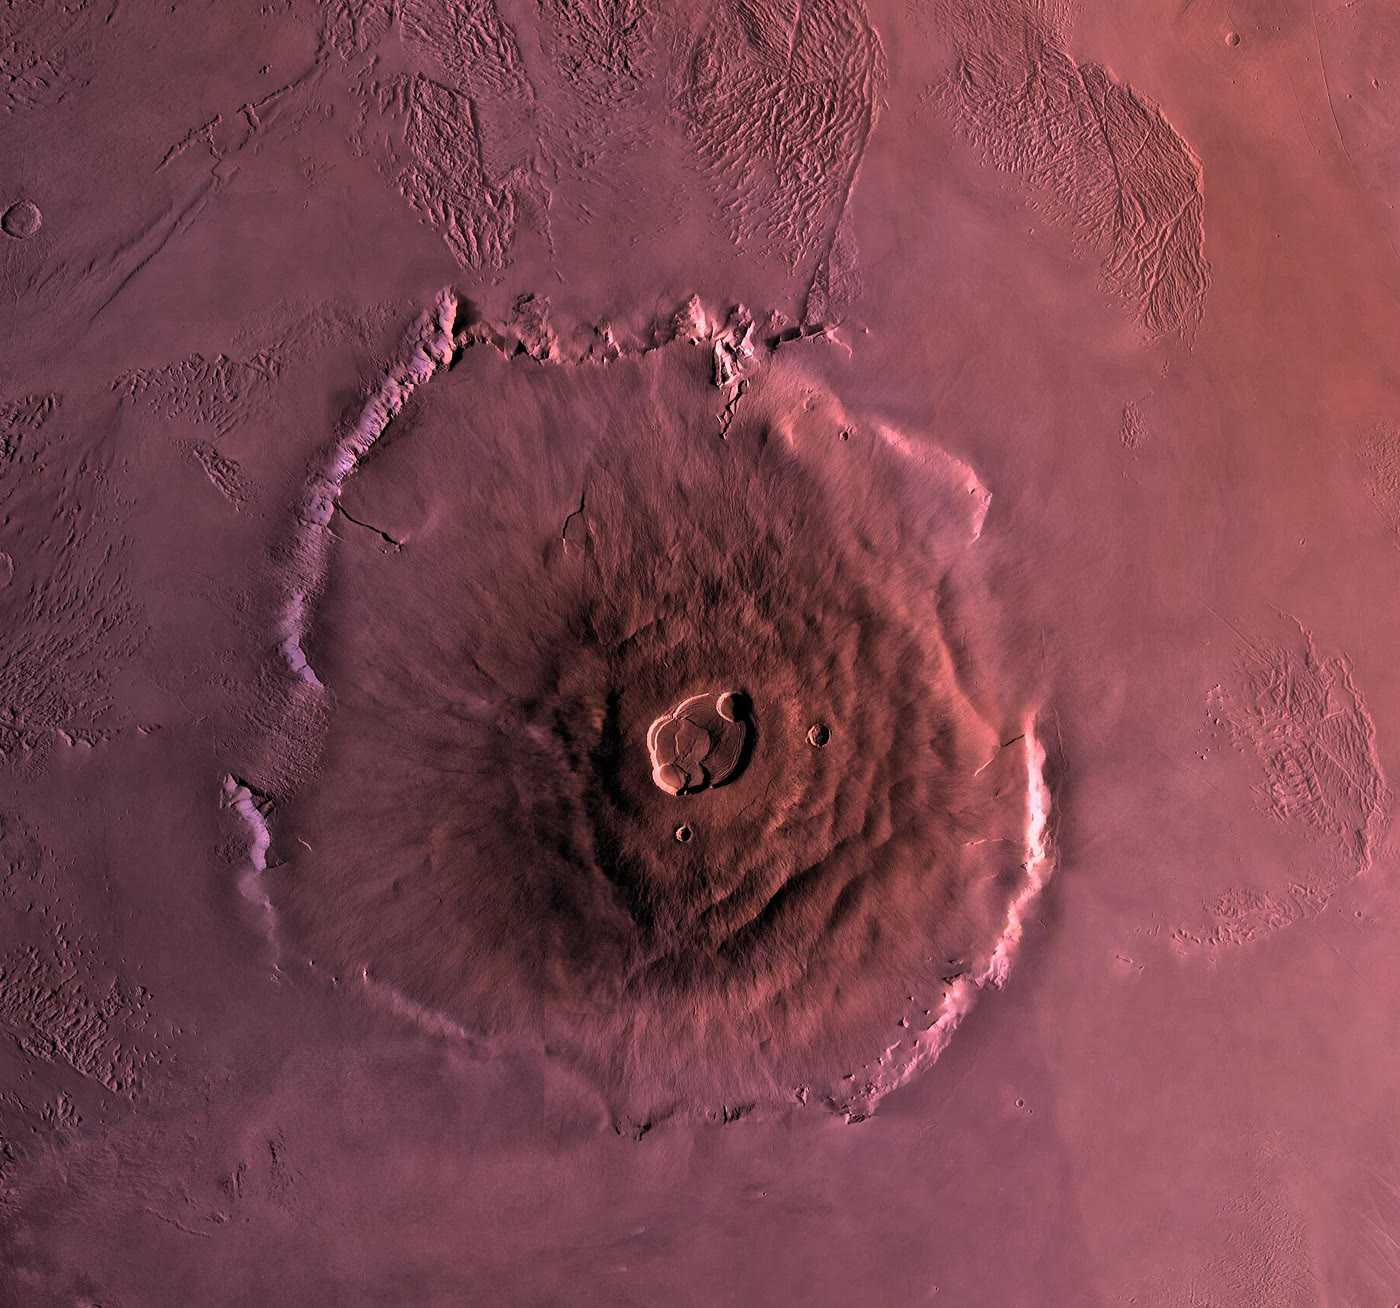
\includegraphics[width=0.48\linewidth]{images/book5/b3-olympus-mons.jpg}
\par\smallskip{\small Monte Olimpo em Marte, um mosaico de imagens das
sondas orbitais Viking: as calderas do cume ao centro, os flancos de fluxos
de lava e a escarpa escalonada que circunda a base, com cerca de \qty{600}{km} de diâmetro.
NASA/JPL/USGS, domínio público.}\label{fig:b3:planetary-interiors-surfaces:olympus}
\end{omfigure}
% ledger: photo:b3-olympus-mons, nasa:olympus-mons

Vênus, gêmeo da Terra em tamanho, tem de longe o menor número de crateras de impacto
de qualquer planeta rochoso, exceto a Terra. Suas feições superficiais podem ter, em média,
apenas 150 milhões de anos, com manchas mais antigas entre elas:
vulcanismo e deformação renovaram a maior parte de sua superfície, talvez
aos poucos ao longo de um longo tempo, talvez mais depressa. Vênus tem milhares de vulcões e nenhum
sinal de placas em movimento.
% ledger: nasa:venus-surface, planet:Venus.diameter, planet:Earth.diameter

Io, a maior lua interna de Júpiter, perde mais de
\qty{2.5}{W.m^{-2}} pela sua superfície, cerca de 27 vezes a média terrestre
de \qty{0.092}{W.m^{-2}}. Seu calor não é o da radioatividade: ele é
produzido pelas marés.
% ledger: veeder:io-heat, dd10:split

\begin{definition}[Aquecimento de maré]\label{def:b3:planetary-interiors-surfaces:tidal-heating}
O \emph{aquecimento de maré}\index{aquecimento de maré} é o calor produzido no interior de um
corpo pelo atrito da deformação que uma maré variável nele impõe.
Uma lua em rotação síncrona, em órbita excêntrica, vê a maré de seu
planeta mudar de intensidade e oscilar de um lado para outro a cada órbita.
\end{definition}

\begin{proposition}[Potência de maré de uma lua síncrona]\label{prop:b3:planetary-interiors-surfaces:tidal-power}
Uma lua de raio $R$ em rotação síncrona, em órbita de movimento médio
$n$ e pequena excentricidade $e$, dissipa a potência
\[
  \dot E = \frac{21}{2}\,\frac{k_2}{Q}\,\frac{(nR)^5}{G}\,e^2 ,
\]
em que $Q$ é o fator de qualidade de maré da lua, de modo que $k_2/Q$ mede a
parte da deformação de maré perdida como calor.
\end{proposition}

A proposição é admitida. As marés que dissipam energia também arredondam
uma órbita; a de Io permanece elíptica, com excentricidade 0.004, porque os puxões
de Europa e Ganimedes, sincronizados com precisão, a perturbam; seus períodos orbitais de
1.77, 3.55 e \num{7.15}~dias ficam quase exatamente na razão
1:2:4 (\cref{exo:b3:planetary-interiors-surfaces:8}). Sua superfície sobe
e desce até \qty{100}{m} a cada órbita. Os vulcões recobrem Io com lava
mais depressa do que as crateras se formam nela; um modelo
de como seu calor escapa é o \omterm{def:b3:planetary-interiors-surfaces:heat-pipe}{vulcanismo de tubo de calor}, que manteria uma litosfera espessa,
fria sob sua superfície incandescente.
% ledger: nasa:galilean-orbits, beuthe:tidal-power, nasa:io-orbit, nasa:io-facts

\begin{definition}[Oceano subsuperficial]\label{def:b3:planetary-interiors-surfaces:ocean-world}
Um \emph{oceano subsuperficial}\index{oceano subsuperficial} é uma camada global de
água líquida sob a casca de gelo de uma lua ou planeta anão, mantida líquida
pelo calor de maré e pelo calor radiogênico.
\end{definition}

\begin{definition}[Criovulcanismo]\label{def:b3:planetary-interiors-surfaces:cryovolcanism}
O \emph{criovulcanismo}\index{criovulcanismo} é a erupção de água, salmouras
ou de outros líquidos e vapores voláteis, em vez de rocha fundida, sobre a
superfície gelada de uma lua ou planeta anão.
\end{definition}

A casca de gelo de Europa, medida pelo radiômetro de micro-ondas da sonda Juno
na região que ela sobrevoou, tem em média cerca de \qty{29}{km} de espessura;
abaixo dela jaz um oceano salgado que contém o dobro da água de todos os
oceanos da Terra. Na lua de Saturno Encélado, com apenas cerca de \qty{500}{km}
de diâmetro, a sonda Cassini encontrou em 2005 jatos de grãos de gelo e gás
saindo de fraturas aquecidas perto do polo sul, a cerca de
\qty{400}{m.s^{-1}}. Sua gravidade e a oscilação de sua rotação mostraram que os
jatos provêm de um oceano global, sob uma casca de gelo com 20 a
\qty{25}{km} de espessura, em média, e talvez apenas 1 a \qty{5}{km}
no polo sul.
% ledger: jpl:europa-shell, nasa:europa-ocean, nasa:enceladus

\section{Núcleos grandes e pequenos}\label{sec:b3:planetary-interiors-surfaces:cores}

Os quatro núcleos medidos formam uma família estranha. Em relação ao seu raio, o núcleo da
Terra chega a 0.55 do caminho até a superfície, e o de Marte, a 0.54; o da Lua,
a 0.19; o de Mercúrio, a 0.82. A diferenciação, no volume do segundo ano,
separa metal de silicato dentro de cada corpo, mas não consegue tornar tão
diferentes as proporções de metal. Impactos gigantes conseguem. Acredita-se que
a Lua tenha se formado a partir dos detritos de uma colisão entre um corpo do
tamanho de Marte e a jovem Terra, cerca de 4.5 bilhões de anos atrás; o metal do
impactor se juntou ao núcleo da Terra, e a Lua reuniu sobretudo rocha do manto, daí seu
núcleo pequeno. Impactos semelhantes podem ter arrancado grande parte do manto
silicático de Mercúrio e deixado o planeta rico em ferro cujo núcleo ocupa a maior parte dele.
Os núcleos registram, assim como as crateras, uma história de colisões.
% ledger: data:prem, jpl:insight-interior, nasa:moon-core, agu:mercury-core, french:giant-impacts

\section{Exercícios}

\begin{exercise}[$\star$]\label{exo:b3:planetary-interiors-surfaces:1}
Mercúrio tem densidade média de \qty{5429}{kg.m^{-3}}, fator de momento de
inércia de 0.35 e raio de \qty{2440}{km}. Com um modelo de duas camadas e um manto de
\qty{3300}{kg.m^{-3}}, calcule o raio relativo do núcleo,
seu raio em quilômetros e sua densidade.
\end{exercise}

\begin{exercise}[$\star$]\label{exo:b3:planetary-interiors-surfaces:2}
Um projétil rochoso de \qty{50}{m} de diâmetro, de densidade \qty{3500}{kg.m^{-3}},
atinge a Terra verticalmente a \qty{20}{km.s^{-1}}. Calcule sua massa
e sua energia cinética, em joules e em megatons de explosivo
($\qty{1}{Mt} = \qty{4.2e15}{J}$). Determine o diâmetro de cratera dado pela regra
de vinte diâmetros do projétil.
\end{exercise}

\begin{exercise}[$\star$]\label{exo:b3:planetary-interiors-surfaces:3}
Em uma planície marciana de \qty{100000}{km^2}, contam-se 120 crateras de \qty{1}{km} ou
mais. Calcule $N_1$, seu erro relativo e a idade-modelo da
planície com seu erro.
\end{exercise}

\begin{exercise}[$\star$]\label{exo:b3:planetary-interiors-surfaces:4}
Io, de raio \qty{1821.5}{km}, perde \qty{2.5}{W.m^{-2}}. Calcule sua
perda total de calor e compare-a com a da Terra, \qty{47}{TW}, no total e
por metro quadrado (\qty{0.092}{W.m^{-2}}).
\end{exercise}

\begin{exercise}[$\star\star$]\label{exo:b3:planetary-interiors-surfaces:5}
Marte tem massa de \qty{6.417e23}{kg} e raio de \qty{3389.5}{km}.
(a)~Calcule sua densidade média, sua gravidade superficial e $\rho gR$.
(b)~Tratando-o como uma esfera uniforme incompressível de rigidez
\qty{67}{GPa}, calcule seu \omterm{def:b3:planetary-interiors-surfaces:love-number}{número de Love} $k_2$. (c)~O valor medido é
$0.153 \pm 0.017$. Explique o que a comparação revela.
\end{exercise}

\begin{exercise}[$\star\star$]\label{exo:b3:planetary-interiors-surfaces:6}
Na Terra ($g = \qty{9.8}{m.s^{-2}}$), a transição de \omterm{def:b3:planetary-interiors-surfaces:crater-morphology}{cratera simples} para
complexa ocorre a cerca de \qty{4}{km} em rocha cristalina e \qty{2}{km} em
sedimentos. (a)~Supondo que o diâmetro de transição varie com $1/g$,
preveja-o para a Lua ($g = \qty{1.62}{m.s^{-2}}$) e para Marte e
Mercúrio ($g = \qty{3.7}{m.s^{-2}}$); compare com os \qty{20}{km}
observados na Lua. (b)~Se o colapso começa quando $\rho gD/3$ supera a
resistência $Y$ da rocha, que valor de resistência dá a transição
cristalina da Terra, para $\rho = \qty{2600}{kg.m^{-3}}$?
\end{exercise}

\begin{exercise}[$\star\star$]\label{exo:b3:planetary-interiors-surfaces:7}
Uma superfície tem $\num{2.0e-3}$ crateras de \qty{1}{km} ou mais por
quilômetro quadrado. Determine sua idade-modelo com a função de cronologia de Marte,
resolvendo a equação numericamente. Que idade a função lunar teria fornecido,
e por que as duas não podem ser trocadas?
\end{exercise}

\begin{exercise}[$\star\star$]\label{exo:b3:planetary-interiors-surfaces:8}
Os períodos orbitais de Io, Europa e Ganimedes são 1.769138, 3.551181 e
\num{7.154553}~dias. (a)~Calcule as razões entre períodos sucessivos.
(b)~Calcule $1/P_I - 3/P_E + 2/P_G$ e comente. (c)~Por que as ressonâncias podem
manter uma excentricidade que as marés, de outra forma, eliminariam?
\end{exercise}

\begin{exercise}[$\star\star$]\label{exo:b3:planetary-interiors-surfaces:9}
Io orbita Júpiter em \num{1.769138}~dias, com excentricidade 0.004.
Calcule a potência que a proposição sobre potência de marés fornece por unidade de $k_2/Q$,
e o valor de $k_2/Q$ que supriria a perda de calor de Io
dada no \cref{exo:b3:planetary-interiors-surfaces:4}.
\end{exercise}

\begin{exercise}[$\star\star\star$]\label{exo:b3:planetary-interiors-surfaces:10}
Para a Lua, $\bar\rho = \qty{3340}{kg.m^{-3}}$ e $C = 0.394$.
(a)~Mostre que, no modelo de duas camadas, $\mathrm dx^2/\mathrm dC =
\tfrac52\bar\rho/(\bar\rho - \rho_m)$ com $\rho_m$ fixo. (b)~Com a
densidade do manto que dá um núcleo de $x = 0.19$, \qty{3288}{kg.m^{-3}},
quais são $x$ e $\rho_c$ quando $C = 0.395$, e quando $C = 0.393$?
(c)~O que isso diz sobre pesar um núcleo pequeno com o momento de
inércia?
\end{exercise}

\begin{exercise}[$\star\star\star$]\label{exo:b3:planetary-interiors-surfaces:11}
(a)~Para 100 crateras, calcule o erro de contagem da idade-modelo de uma
superfície marciana de \qty{1.0}{Ga} e de outra de \qty{3.8}{Ga}.
(b)~Mostre que, na parte linear da função de cronologia, $\sigma_T/T =
1/\sqrt n$. (c)~Por que, então, as idades de superfícies antigas continuam incertas?
\end{exercise}

\begin{exercise}[$\star\star\star$]\label{exo:b3:planetary-interiors-surfaces:12}
Europa, de raio \qty{1560.8}{km}, orbita em \num{3.551181}~dias, com
excentricidade 0.009. (a)~Se Europa dissipasse marés com o mesmo $k_2/Q$
como Io, qual fração da potência de maré de Io ela produziria, e qual seria o fluxo de calor?
(b)~Por que essa hipótese é duvidosa para uma lua com um oceano sob o gelo?
\end{exercise}

\section{Problema: duas planícies em Marte}

\begin{problem}[{Problema de fim de semana --- o núcleo de Marte e as idades de duas
planícies de lava inventadas}]
\label{pb:b3:planetary-interiors-surfaces:1}
Marte tem massa de \qty{6.4169e23}{kg}, raio de \qty{3389.5}{km} e um
fator de momento de inércia de 0.366. Duas planícies inventadas, A e B, situam-se
sobre suas províncias vulcânicas; suas crateras foram contadas em imagens, em classes
com largura $\sqrt2$.

\medskip\noindent\textbf{Parte I --- O núcleo.}
\begin{enumerate}
\item Calcule a densidade média de Marte.
\item Com um modelo de duas camadas e um manto de \qty{3500}{kg.m^{-3}}, calcule
  o raio relativo do núcleo, seu raio em quilômetros e sua
  densidade.
\item A missão InSight mediu um raio de núcleo de \qty{1830}{km}. Quais densidades de manto e de núcleo
  o modelo de duas camadas então exige?
\item Compare essa densidade do núcleo com a densidade do núcleo externo da Terra
  logo abaixo do topo, \qty{9900}{kg.m^{-3}} no modelo de referência da Terra,
  e diga por que se espera um valor menor para Marte, e o que mais isso
  sugere.
\item O \omterm{def:b3:planetary-interiors-surfaces:love-number}{número de Love} da esfera uniforme de Marte, com rigidez de
  \qty{67}{GPa} é 0.109; o medido é 0.153. Qual observação veio
  primeiro, e o que ela já dizia sobre o núcleo?
\item A crosta de Marte tem de 20 a \qty{37}{km} de espessura. Que fração do
  volume do planeta ela ocupa? Foi correto desprezá-la?
\end{enumerate}

\medskip\noindent\textbf{Parte II --- A contagem na planície A.} A planície A
cobre \qty{80000}{km^2}. Suas crateras, por classe de diâmetro (km):
\begin{center}
\small
\begin{tabular}{lccccccccc}
\hline
classe & 1--1.41 & 1.41--2 & 2--2.83 & 2.83--4 & 4--5.66 & 5.66--8 & 8--11.3 & 11.3--16 & 16--22.6 \\
\hline
planície A & 38 & 6 & 5 & 3 & 0 & 0 & 0 & 1 & 1 \\
planície B & 48 & 8 & 31 & 12 & 7 & 2 & 0 & 2 & 2 \\
\hline
\end{tabular}
\end{center}
\begin{enumerate}[resume]
\item Calcule as contagens acumuladas da planície A, a partir de \qty{1}{km}.
\item Calcule $N(\qty{1}{km})$ por quilômetro quadrado e seu desvio
  padrão.
\item A função de produção fornece $F(\qty{2}{km}) = 0.147$ e
  $F(\qty{1.41}{km}) = 0.355$. As contagens em 1.41 e \qty{2}{km}
  são consistentes com a forma da função de produção?
\item A planície A está em algum ponto próximo da densidade de equilíbrio,
  \qty{0.072}{km^{-2}} em \qty{1}{km}?
\item Por que as classes são escolhidas com largura $\sqrt2$?
\item Aglomerados e cadeias de pequenas crateras ficam de fora de uma contagem. Por quê?
\end{enumerate}

\medskip\noindent\textbf{Parte III --- Idades-modelo.} Use a
função de cronologia de Marte.
\begin{enumerate}[resume]
\item Calcule a idade-modelo da planície A. Verifique que o termo exponencial
  pode ser desprezado.
\item Calcule seu erro de contagem.
\item Qual idade a cronologia lunar teria fornecido?
\item A planície B cobre \qty{120000}{km^2}. Usando suas crateras de \qty{2}{km}
  e maiores, calcule $N(\qty{2}{km})$, depois $N_1$ e, por fim, sua idade-modelo,
  resolvendo a equação numericamente.
\item Calcule o erro de contagem dessa idade.
\item Compare os erros relativos das duas idades e explique a
  diferença.
\end{enumerate}

\medskip\noindent\textbf{Parte IV --- As crateras enterradas da planície B.}
\begin{enumerate}[resume]
\item Quantas crateras entre \num{1} e \qty{2}{km} a planície B deveria conter se
  toda a sua superfície tivesse a idade da questão~16? Quantas ela contém de fato?
\item Suponha que a lava tenha enterrado todas as crateras menores que \qty{2}{km} num
  instante $T_r$ e poupado as maiores. Calcule $T_r$ a partir das
  crateras de \num{1}--\qty{2}{km}.
\item Calcule o erro de contagem de $T_r$.
\item Tome uma \omterm{def:b3:planetary-interiors-surfaces:crater-morphology}{cratera simples} recente em Marte como tendo profundidade igual a um quinto de sua
  largura (uma hipótese deste problema). Qual deve ser a espessura da lava para enterrar
  uma cratera de \qty{2}{km}, e por que as maiores ainda aparecem?
\item A lava da planície B e a da planície A poderiam pertencer a um único episódio
  de vulcanismo?
\item Dê a idade-modelo da planície A, em bilhões de anos, com dois
  algarismos significativos.
\end{enumerate}
\end{problem}
% ledger: nasa:mars, jpl:insight-interior, yoder:mars-k2, data:prem, craterstats:mars-pf, craterstats:mars-cf, craterstats:moon-cf, craterstats:equilibrium
